\chapter{Formal Analysis}
In this chapter the Alloy model of the CKB system is implemented, describing the main constraints and focusing in particular on the consistency of the world.\\
\lstinputlisting[language=alloy]{alloy/alloy.als}

The following figures show the evolution of a tournament: starting as available, then the registration deadline expires and it becomes active; 
then a battle is created and once its registration deadline expires it becomes active too. When the submission deadline ends, the battle closes. 
Finally, the tournament ends. 

\begin{figure}[H]
    \centering
    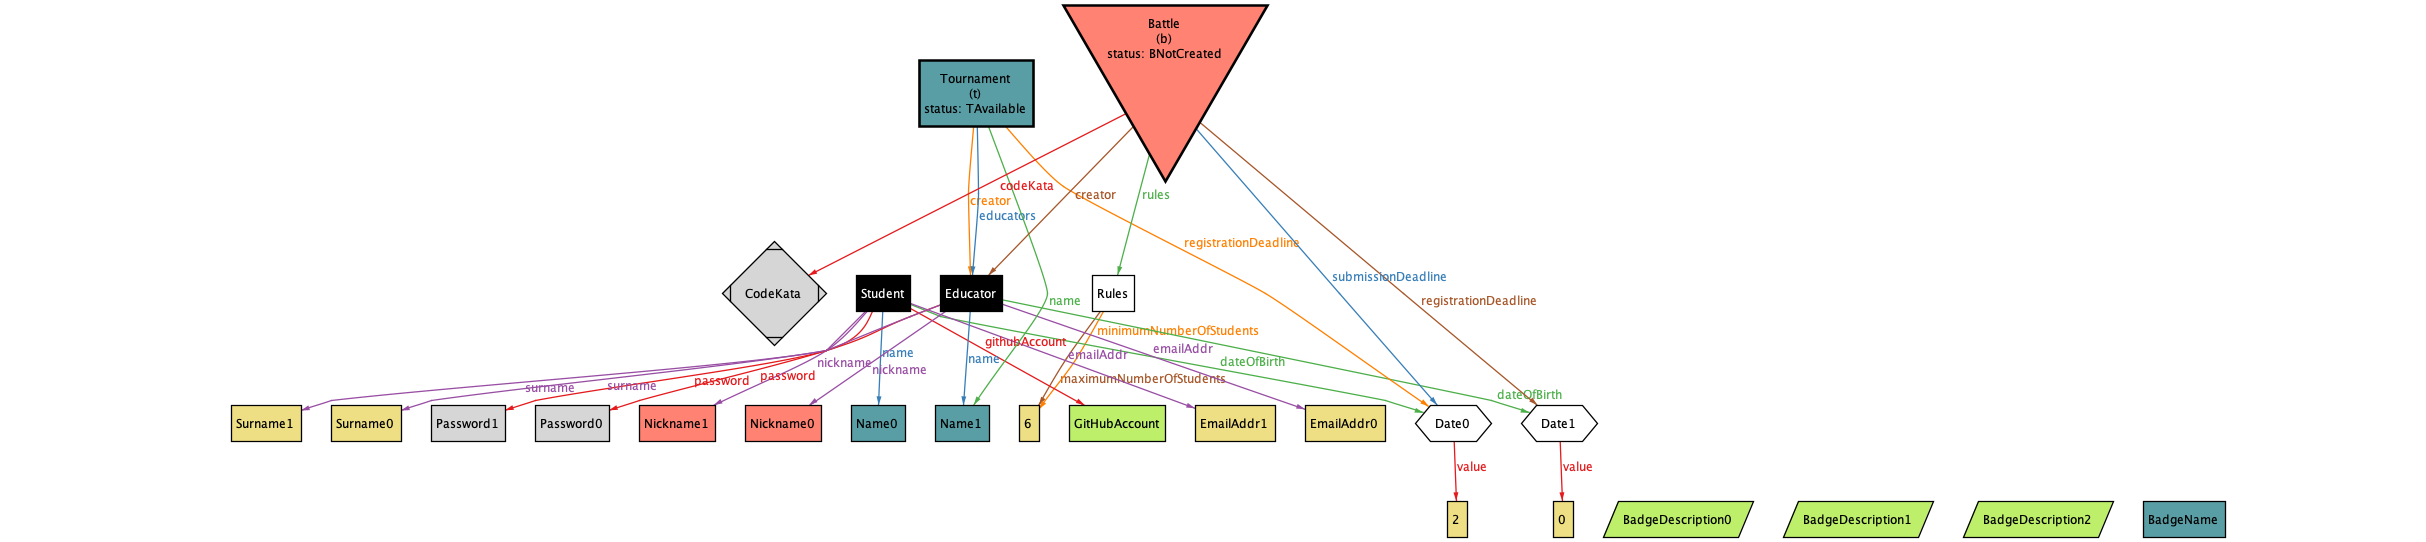
\includegraphics[angle=90,origin=c, height=0.91\textwidth]{alloy/images/example1_0.png}
    \caption{Example 1 - Instant 0}
\end{figure}

\begin{figure}[H]
    \centering
    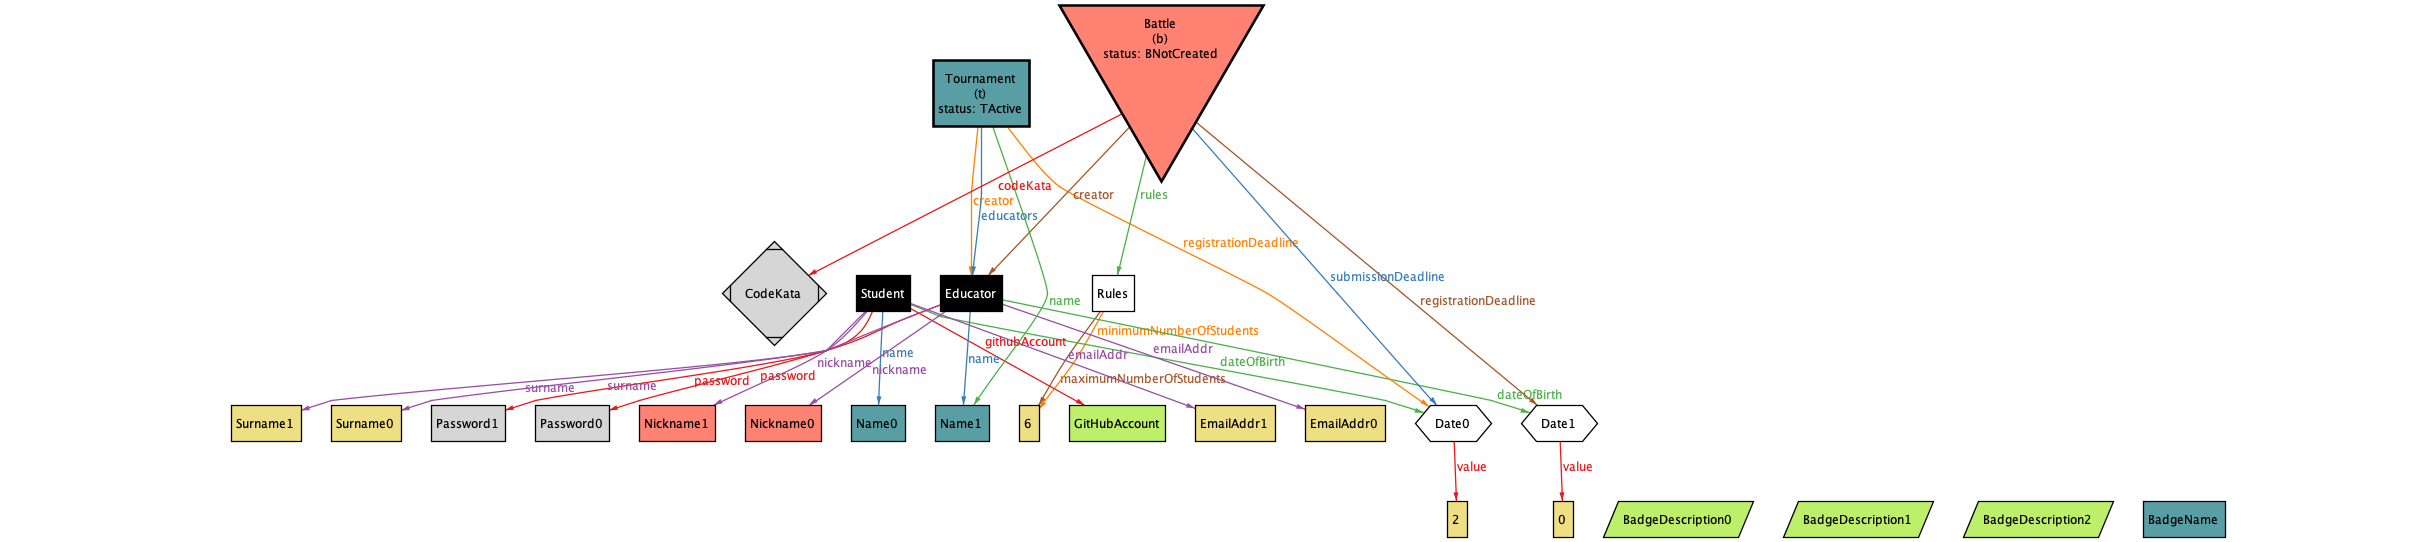
\includegraphics[angle=90,origin=c, height=0.91\textwidth]{alloy/images/example1_1.png}
    \caption{Example 1 - Instant 1}
\end{figure}

\begin{figure}[H]
    \centering
    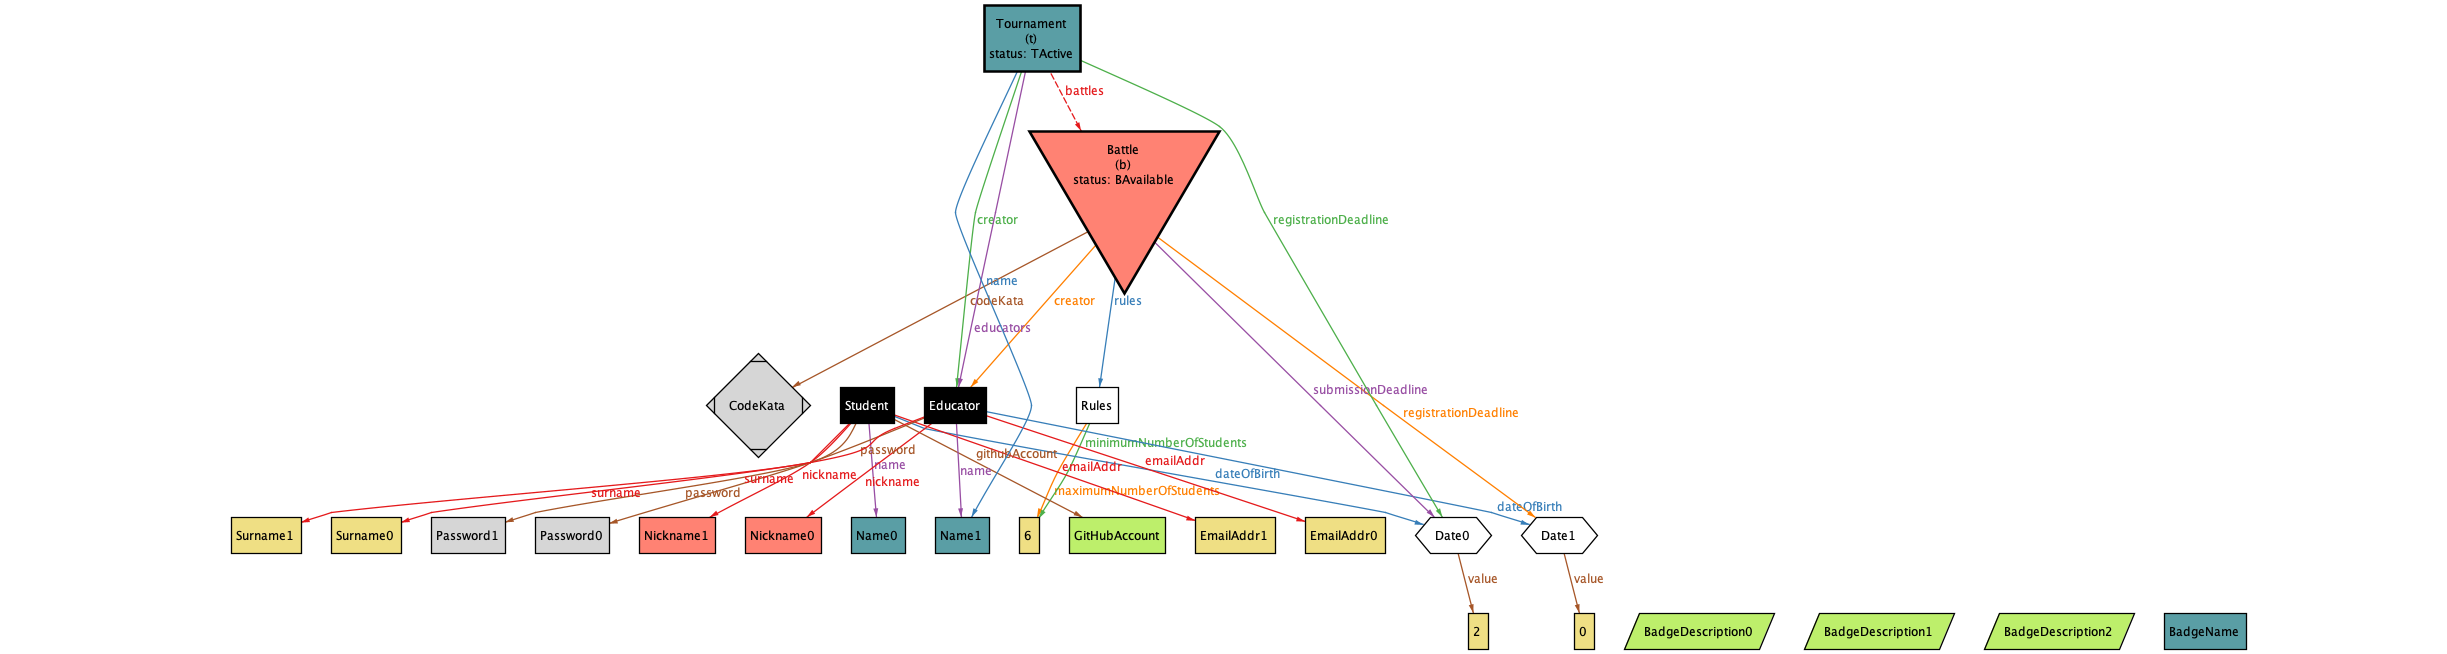
\includegraphics[angle=90,origin=c, height=0.91\textwidth]{alloy/images/example1_2.png}
    \caption{Example 1 - Instant 2}
\end{figure}

\begin{figure}[H]
    \centering
    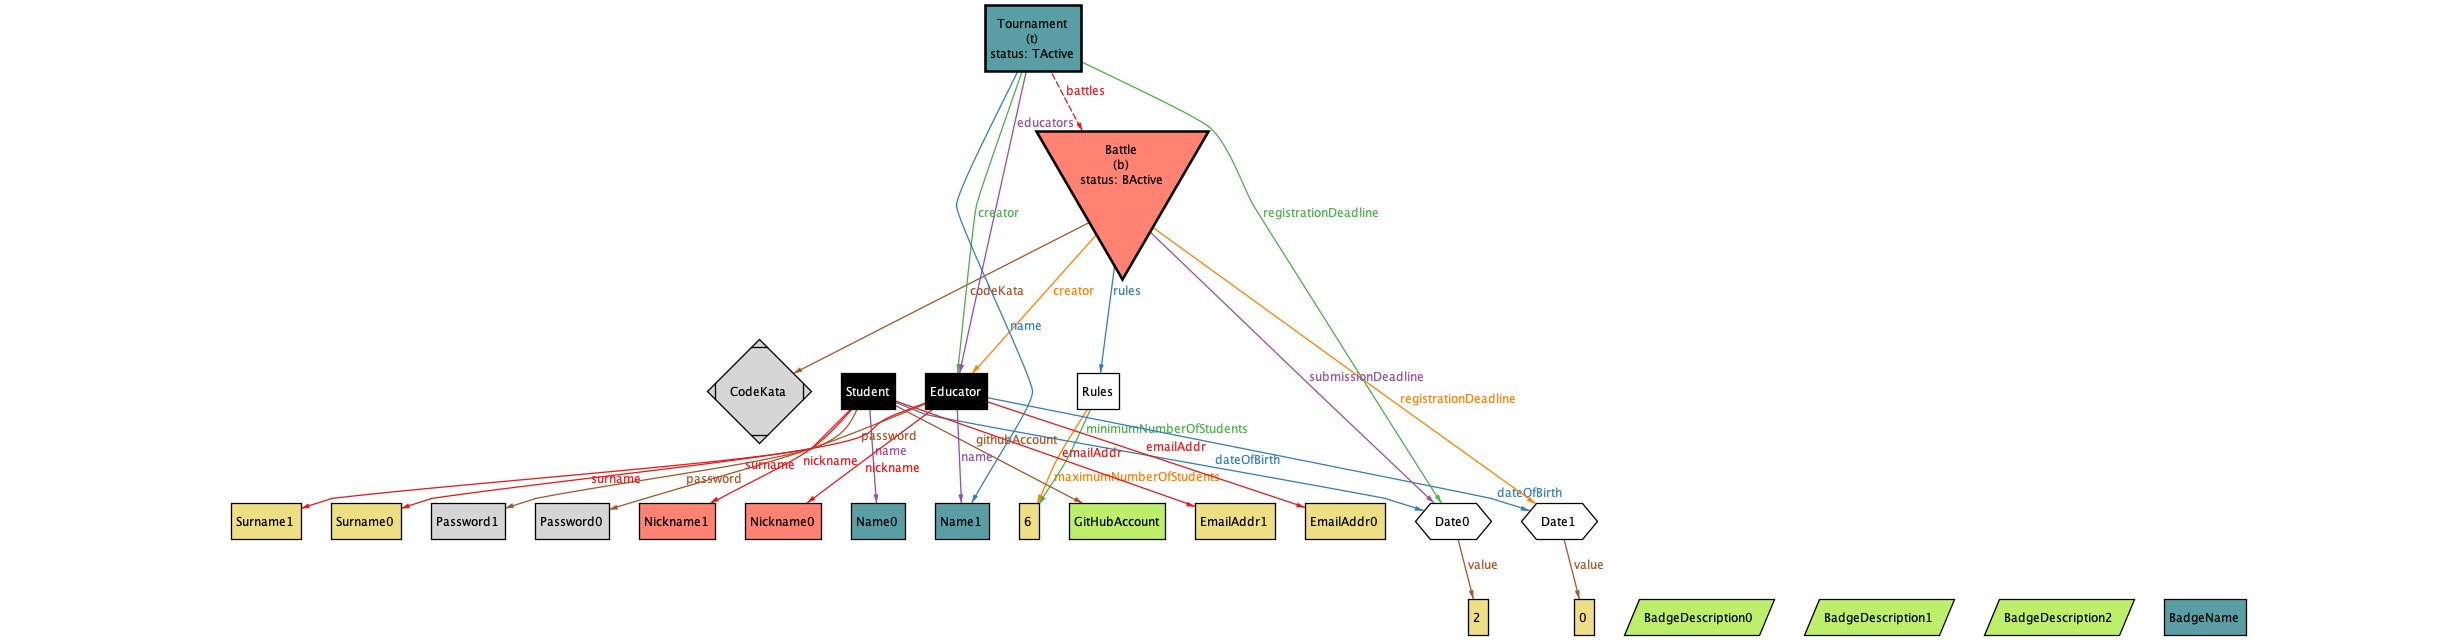
\includegraphics[angle=90,origin=c, height=0.91\textwidth]{alloy/images/example1_3.png}
    \caption{Example 1 - Instant 3}
\end{figure}

\begin{figure}[H]
    \centering
    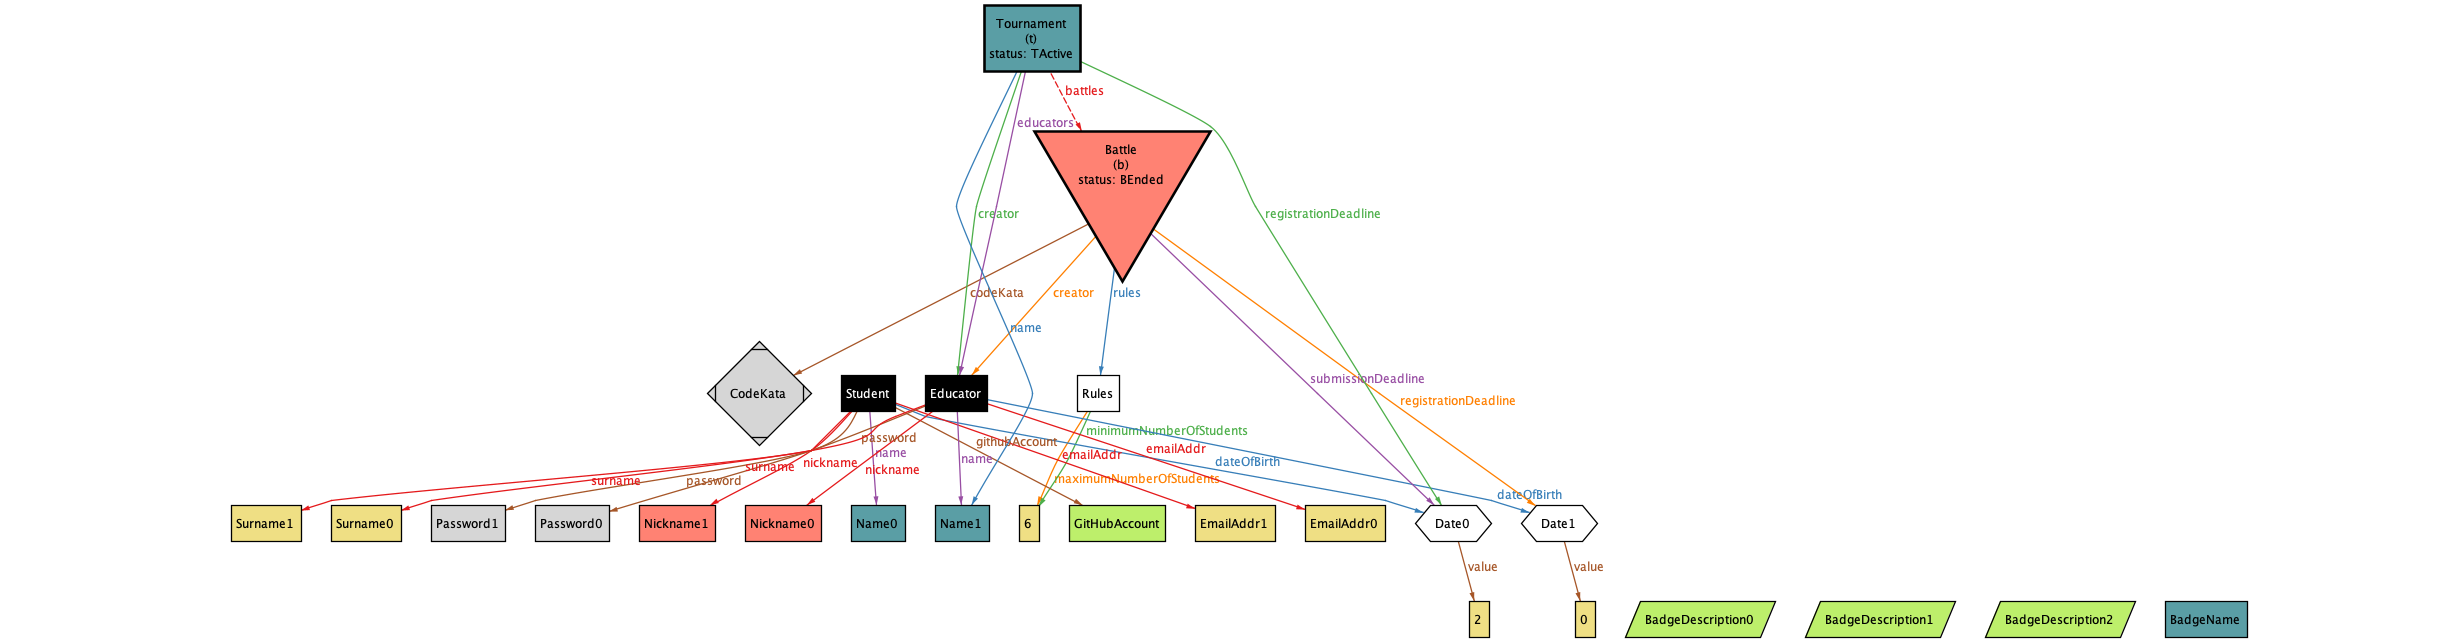
\includegraphics[angle=90,origin=c, height=0.91\textwidth]{alloy/images/example1_4.png}
    \caption{Example 1 - Instant 4}
\end{figure}

\begin{figure}[H]
    \centering
    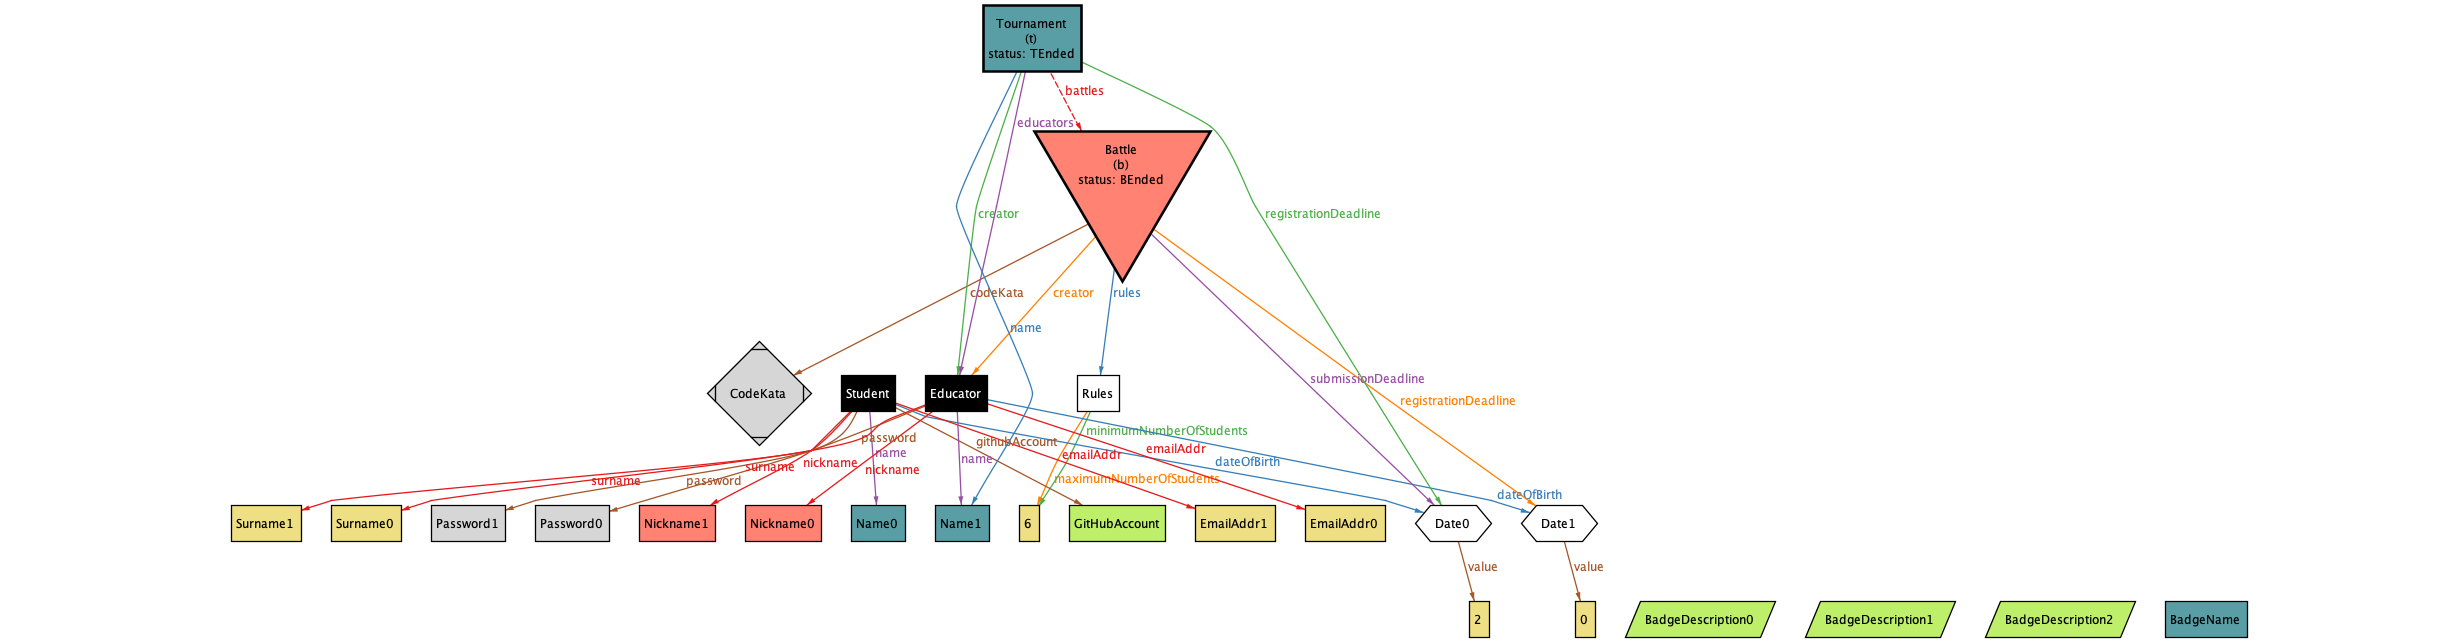
\includegraphics[angle=90,origin=c, height=0.91\textwidth]{alloy/images/example1_5.png}
    \caption{Example 1 - Instant 5}
\end{figure}